\documentclass[ba]{imsart}

% \documentclass[ba,preprint]{imsart}% use this for supplement article
\usepackage{amsmath}
\usepackage{amssymb}
\usepackage{amsfonts}
\usepackage{amsthm}
%% \usepackage{amsaddr}


\theoremstyle{plain}
\newtheorem{theorem}{Theorem}
\newtheorem{corollary}[theorem]{Corollary}
\newtheorem{lemma}[theorem]{Lemma}
\newtheorem{proposition}[theorem]{Proposition}
\theoremstyle{definition}
\newtheorem{definition}[theorem]{Definition}
\newtheorem{example}[theorem]{Example}
\newtheorem{conjecture}[theorem]{Conjecture}
\theoremstyle{remark}
\newtheorem{remark}[theorem]{Remark}

\usepackage{thm-restate}
\usepackage{tikz,pgfplotstable}
\usetikzlibrary{patterns}
\pgfplotsset{compat=1.9} % set to 1.8 to get old behaviour
%\usepackage{hyperref}

\newcommand{\R}{\ensuremath{\mathbb{R}}}
\newcommand{\eps}{\varepsilon}
\newcommand{\M}{\mathcal{M}}

\newcommand{\der}{\text{\textup{d}}}
\newcommand{\diag}{\textup{diag}}

\providecommand{\x}{}
\renewcommand{\x}{\mathbf{x}}
\newcommand{\y}{\mathbf{y}}

\newcommand{\hil}{\mathcal{H}}
\newcommand{\hilp}{\mathcal{H}_p}
\newcommand{\hilo}{\mathcal{H}_o}
\newcommand{\obs}{\mathcal{O}}
\newcommand{\pobs}{\mathcal{P}}
\newcommand{\fwd}{\mathcal{F}}

\newcommand{\obsm}{\widehat{\obs}}
\newcommand{\Sigmam}{\widehat{\Sigma}}
\newcommand{\postcovm}{\widehat{\Gamma_{\textup{post}}}}
\newcommand{\uu}{\mathbf{u}}
\newcommand{\tar}{\Psi}
\DeclareMathOperator*{\argmin}{arg\,min}
\DeclareMathOperator*{\argmax}{arg\,max}

% Definitions for second chapter
\newcommand{\data}{\mathbf{d}}
\newcommand{\param}{\mathbf{m}}
\newcommand{\normal}{\mathcal{N}}
\newcommand{\pr}{\mu_{\textup{pr}}} %Prior measure
\newcommand{\post}{\mu_{\textup{post}}^{\data, \obs}} % Posterior measure
\newcommand{\prmean}{\param_{\textup{pr}}} % Prior mean
\newcommand{\postmean}{\param_{\textup{post}}} % Posterior mean
\newcommand{\postcov}{\Gamma_{\textup{post}}} % Posterior covariance
\newcommand{\prcov}{\Gamma_{\textup{pr}}} % Prior covariance
\newcommand{\modcov}{\Gamma_{\textup{model}}} % Model covariance
\newcommand{\tmp}{\mathcal{G}}
\newcommand{\meas}{\mathbf{o}}
\newcommand{\ev}{\mathbf{e}} % eigenvector 
\newcommand{\func}{\mathbf{a}}
\newcommand{\tr}[1]{\textup{tr}\left \{#1 \right \} }
\newcommand{\ttr}[1]{\textup{tr}\ #1}
\newcommand{\rank}{\textup{rank}\ }
\newcommand{\des}{\eta} % vector of design parameters
\newcommand{\sigsqr}{\sigma^2}


%% %\usepackage{comment}% http://ctan.org/pkg/comment
%% %% %% %\excludecomment{proof}
%% %% \excludecomment{figure}
%% %% \let\endfigure\relax


%% %\overfullrule=0pt

%
\pubyear{2021}
\volume{TBA}
\issue{TBA}
% \doi{0000}
%\arxiv{}
\firstpage{1}
\lastpage{1}

\usepackage{amsthm}
\usepackage{amsmath}
\usepackage{natbib}
\usepackage[colorlinks,citecolor=blue,urlcolor=blue,filecolor=blue,backref=page]{hyperref}
\usepackage{graphicx}

\startlocaldefs
% ** Local definitions **
\endlocaldefs

\begin{document}

%% *** Frontmatter *** 

\begin{frontmatter}
\title{Measurement Clusterization in Bayesian D-optimal Designs in Infinite Dimensions}

%\title{\support{}}
\runtitle{Measurement Clusterization in D-optimal Designs}
%\author{Yair Daon}
%\numberwithin{equation}{section}

\begin{aug}
\author{\fnms{Yair} \snm{Daon}\thanksref{addr1}\ead[label=e1]{yair.daon@gmail.com}}
\runauthor{Yair Daon}

\address[addr1]{Azrieli Faculty of Medicine, Bar-Ilan University, Safed, Israel
    \printead{e1} % print email address of "e1"
}

\end{aug}

\begin{abstract}
Estimation of parameters in physical processes often demands costly measurements, prompting the pursuit of an optimal measurement strategy. Finding such strategy is termed the problem of \emph{optimal experimental design}, abbreviated as optimal design. Remarkably, optimal designs can yield tightly clustered measurement locations, leading researchers to fundamentally revise the design problem just to circumvent this issue. Some authors introduce error correlation among error terms that are initially independent, while others restrict measurement locations to a finite set of locations. While both approaches may prevent clusterization, they also fundamentally alter the optimal design problem.

In this study, we consider Bayesian D-optimal designs, i.e.~designs that maximize the expected Kullback-Leibler divergence between posterior and prior. We propose an analytically tractable model for D-optimal designs over Hilbert spaces. In this framework, we make several key contributions: \textbf{(a)} We establish that measurement clusterization is a generic trait of D-optimal designs with independent Gaussian measurement errors, and prove that introducing correlations among measurement error terms mitigates clusterization. \textbf{(b)} We characterize D-optimal designs as reducing uncertainty across a subset of prior covariance eigenvectors. Finally, \textbf{(c)} We leverage this characterization to argue that measurement clusterization arises as a consequence of the pigeonhole principle: when more measurements are taken than there are locations where the select eigenvectors are large and others are small --- clusterization occurs. 
%
%% In summary, in this study we shed light on an often ignored issue with
%% Bayesian D-optimal designs. We characterize such designs and show why
%% clusterization arisesit arisestheir inherent properties, propose
%% strategies to address clusterization, and provide insights into the
%% fundamental attributes underlying measurement design optimization.
\end{abstract}

%% ** Keywords **
\begin{keyword}[class=MSC]
\kwd[Primary ]{62F15}
\kwd{35R30}
\kwd[; secondary ]{28C20}
\end{keyword}

\end{frontmatter}

\section{Introduction}\label{section:intro}
Measurements play a fundamental role in generating observations and
are indispensable to any inference process. Selecting the optimal set
of measurements holds particular significance when inferring
parameters of a physical process. Unlike many other fields, where
measurements are fixed, in this context, we have the freedom to choose
which measurements to take. This freedom should be taken advantage of:
measurements should be chosen to enhance accuracy, reduce costs, or
both. Whether measurements involve specifying electrode locations on
the skin in electric impedance tomography \cite{horesh2010impedance},
determining certain wavelengths in MRI \cite{horesh2008mri},
positioning sensors for detecting ground-reflected waves in the search
for oil \cite{horesh2008borehole}, or optimizing sensor locations in a
seismographic network \cite{rabinowitz1990, steinberg1995} --- the
selection of optimal measurements, referred to as the problem of
\emph{optimal design}, becomes crucial. Optimal measurements are
chosen according to specific \emph{design criteria}, with A- and
D-optimality being two of the most widely recognized and extensively
studied design criteria \cite{Chaloner1995,
  AlexanderianGloorGhattas14}.


Surprisingly, A- and D-optimal designs have been observed to yield
remarkably similar measurements in certain cases \cite{fedorov1996,
  nyberg2012, fedorov1997, Ucinski05, neitzel2019sparse}. To
illustrate this point, we consider a toy problem: inferring the
initial condition of the 1D heat equation (details in the
supplementary material). In Fig.~\ref{fig:clusterization_illustration}
D-optimal measurement locations are shown for different numbers of
measurements. Notably, for six measurements, a D-optimal design yields
two sets of measurements that are almost indistinguishable from one
another. We refer to this intriguing phenomenon as \emph{measurement
clusterization} \cite{Ucinski05}, and we refer to a design that
exhibits measurement clusterization as a \emph{clustered design}.


%% first: blue, second: red, third: green, fourth: black,
%% fifth:magenta
\begin{figure}
    \centering
    \includegraphics[height=0.5\textwidth]{figs/example.png}
    \caption{Measurement clusterization for optimal designs when
      inverting for the initial condition of the 1D heat equation (see
      supplementary material for details). Measurement locations were
      chosen according to the Bayesian D-optimality criterion of
      Theorem \ref{thm:d_optimality}. Measurement locations are
      plotted over the computational domain \(\Omega = [0, 1]\)
      (x-axis), for varying numbers of measurements (y-axis). The
      colored numbers are measurement indices, plotted for visual
      clarity. Measurement clusterization already occurs for three
      measurements: the second measurement (red) is overlaid with the
      third (green). For five measurements, first (blue) and second
      (red) measurements are clustered, as well as the fourth (black)
      and the fifth (magenta).}
  \label{fig:clusterization_illustration}
\end{figure}


Researchers widely agree that measurement clusterization is
undesirable \cite{fedorov1996, nyberg2012, fedorov1997, Ucinski05,
  neitzel2019sparse}, prompting the exploration of various remedies to
address this issue. One approach involves merging close measurements
\cite{fedorov1997}; however, this strategy merely overlooks the
phenomenon of measurement clusterization. An alternative solution lies
in \emph{clusterization-free design}s, where measurement locations are
deliberately chosen to be distant from one another. This can be
achieved by imposing distance constraints between measurements or by
introducing correlated errors that account for both observation error
and model misspecification \cite{Ucinski05}. For instance, in the
context of time-series analysis for pharmacokinetic experiments,
measurement clusterization can be mitigated by incorporating the
modeling of auto-correlation time within the noise terms
\cite{nyberg2012}.


In spatial problems involving choice of measurements within a domain
\(\Omega \subseteq \mathbb{R}^d, d=1,2,3\), many researchers
circumvent the problem of measurement clusterization by choosing
measurements from a coarse grid in \(\Omega\) \cite{koval2020,
  alexanderian2021, attia2022, alexanderian2014, alexanderian2016,
  alexanderian2018efficient, brunton2016}. This approach incurs a
significant computational cost as it requires solving a difficult
combinatorial optimization problem for measurement locations over a
finite set. The combinatorial optimization problem is usually relaxed
by first assigning optimal measurement weights in \(\mathbb{R}_+\) to
the potential measurement locations. Some researchers incorporate a
sparsifying \(\ell_1\) penalty term into the design criterion, which
is subsequently thresholded to achieve the desired binary design over
the coarse grid \cite{horesh2008borehole}. Others progressively relax
the \(\ell_1\) penalty to an \(\ell_0\) penalty via a continuation
method \cite{alexanderian2016, alexanderian2014}. Others cast the
problem of finding optimal measurement weights as a stochastic
optimization problem \cite{attia2022stochastic}. All of the
aforementioned methods may indeed find a binary optimal design
restricted to a given coarse grid. However, none addresses one
fundamental issue: the restriction of measurement locations to a
coarse grid in \(\Omega\) fundamentally changes the optimal design
problem and thus results in a sub-optimal design.

Avoiding measurement clusterization is a pragmatic approach:
intuitively, researchers recognize that measurement clusterization is
undesirable, even though the underlying reasons may not be fully
clear. Consequently, they strive to prevent it and devise various
methodologies to avoid measurement clusterization. Yet each and every
one of these methodologies achieves its objective by imposing
restrictions on measurement locations, thereby fundamentally altering
the optimal design problem. To the best of my knowledge, no previous
study has tried to address some seemingly simple yet fundamental
questions:
%
Why does imposing correlations between observations alleviate
measurement clusterization?
%
Is measurement clusterization a generic phenomenon?
%
And, most importantly: Why does measurement clusterization occur?
%
%Should we aim to avoid measurement clusterization?
%
%Is it possible to substitute an optimal clustered design with an
%equally optimal non-clustered design?
%Can an optimal clustered design be relpaced with an equally optimal
%non-clustered design?


\subsection{Contribution}
The primary objective of this study is to provide a comprehensive
understanding of measurement clusterization by addressing the
aforementioned questions. Our focus centers around investigating the
Bayesian D-optimality criterion, which involves maximizing the
expected Kullback-Leibler divergence between the posterior and prior
measures \cite{CoverThomas91, Chaloner1995}. We conduct an analysis of
Bayesian D-optimal designs within the context of linear inverse
problems over Hilbert spaces. We propose a novel relaxed model for
D-optimality that maintains analytical tractability and enables the
identification of D-optimal designs using Lagrange multipliers. This
analytical framework facilitates the exploration of the questions
posed at the end of the previous paragraph:

\begin{figure}
    \centering
    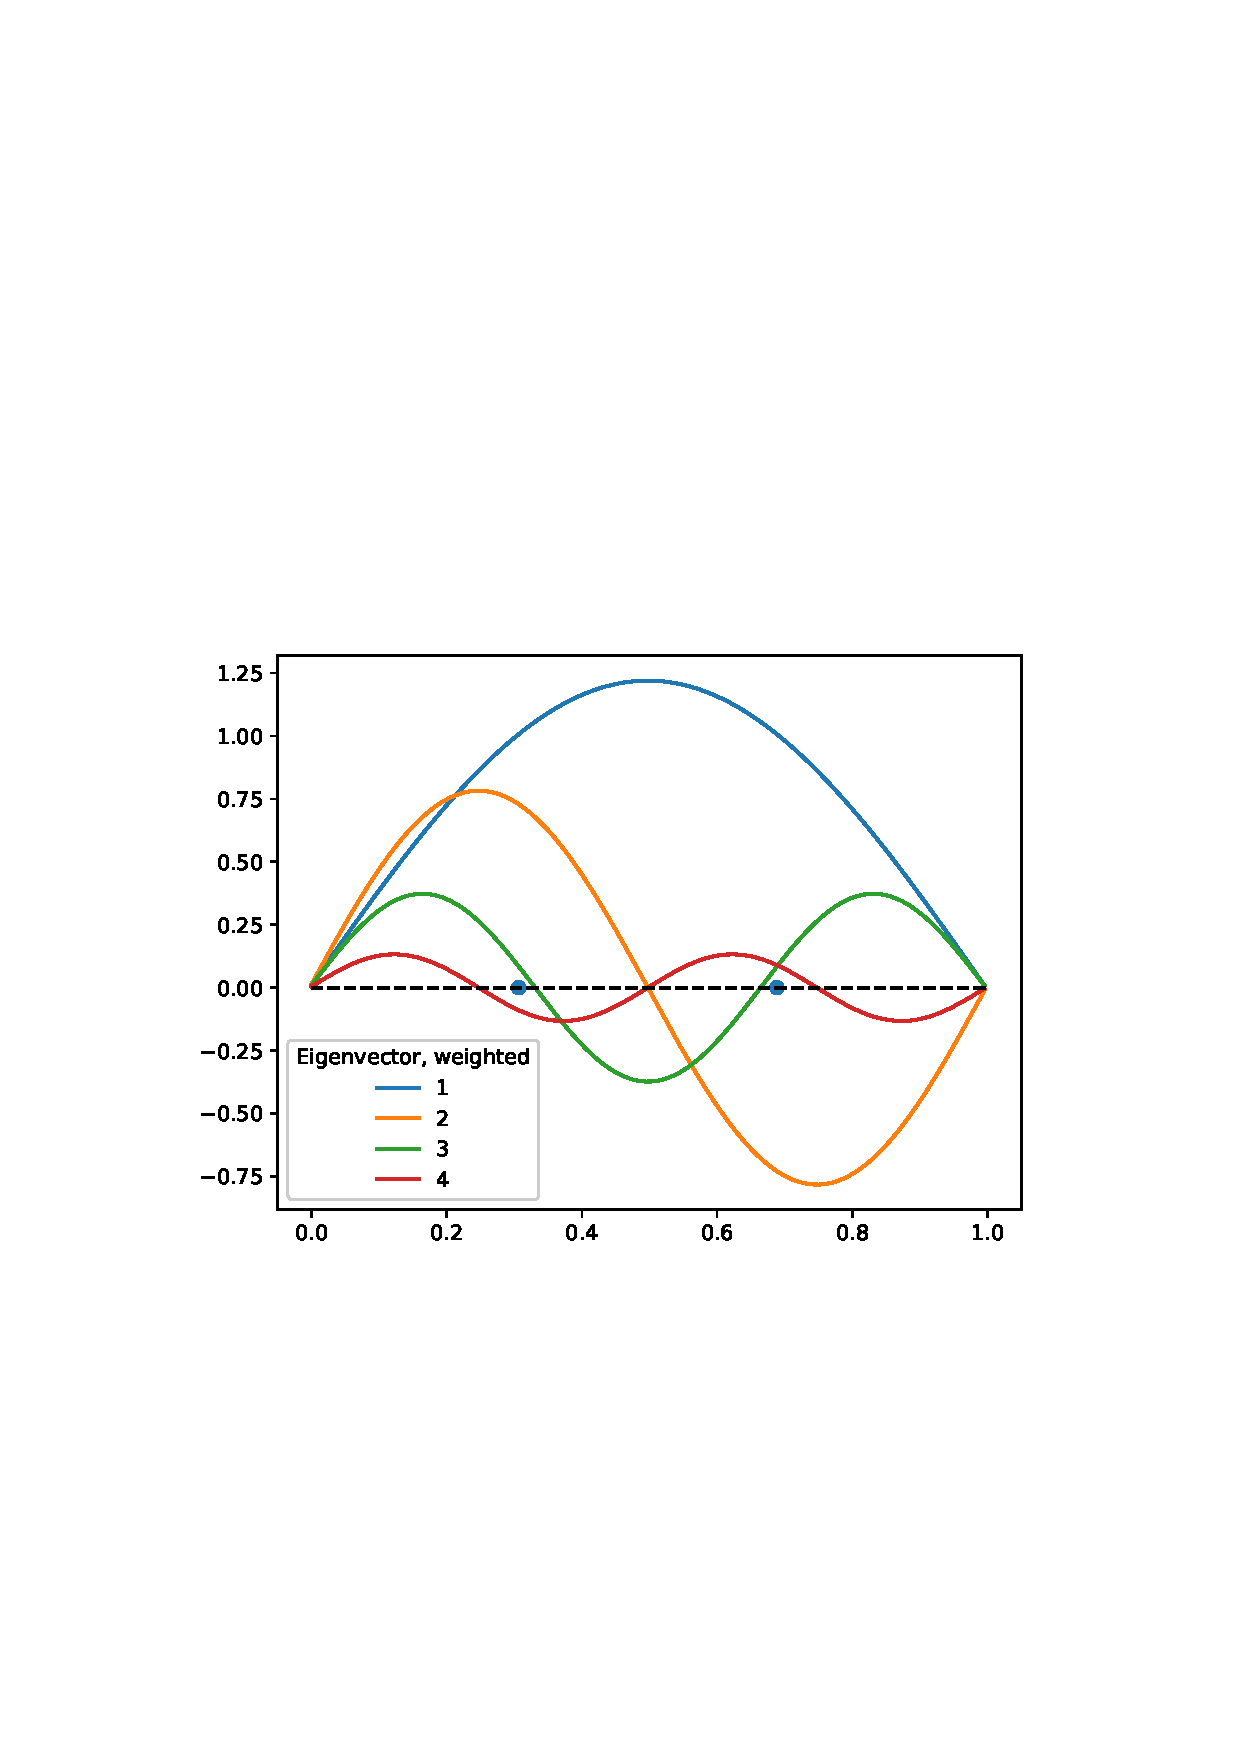
\includegraphics[width=\textwidth]{figs/eigenvectors.png}
    \caption{D-optimal measurement locations ($m=4$ measurements) and
      weighted eigenvectors for finding the initial condition of
      the 1D heat equation. Measurement locations and weighted
      eigenvectors are plotted over the computational domain $\Omega =
      [0, 1]$ (x-axis). Measurement clusterization occurs
      approximately at $0.31$ and $0.69$. These two locations are a
      compromise between zeros of eigenvectors a D-optimal design aims
      to ignore (third and up) and staying far from zeros of the
      eigenvectors a D-optimal design aims to measure (first and
      second). Allocating $m=4$ measurements into two locations
      results in clusterization, according to the pigeonhole
      principle.}
  \label{fig:why}
\end{figure}

\begin{enumerate}

\item \label{q:generic} \textbf{Is measurement clusterization a
  generic phenomenon?}
  %\subsection{An answer for Question \ref{q:generic}: Genericity of measurement clusterization}
  %% Computer implementation of Lemma \ref{thm:char} for the inverse
  %% problem outlined in Section \ref{section:how} also generates \(\obs\)
  %% as a solution to the D-optimal design problem.  Furthermore,
  Randomized numerical simulations of our model give rise to D-optimal
  designs that exhibit clusterization more than 95\% of the time (see
  code in supplementary material). Given our model's genericity, we
  expect measurement clusterization to be a generic phenomenon.

\item \label{q:mitigate} \textbf{Why does imposing correlations
  between observations alleviate measurement clusterization?} In
  Section \ref{section:non_vanishing}, we rigorously demonstrate the
  role of model error in mitigating clusterization, thereby
  corroborating earlier observations made by various researchers.

\item \label{q:why} \textbf{Why does measurement clusterization
  occur?} In Section \ref{section:why}, we present a compelling
  explanation for the optimality of clustered designs in the absence
  of model error. Our analysis reveals that, in our model, a D-optimal
  design focuses on a select set of prior eigenvectors, specifically
  those with the largest eigenvalues in the prior covariance
  spectrum. In practical scenarios, the number of locations where (a)
  the relevant prior eigenvectors are significantly large, and (b)
  other eigenvectors are close to zero, is limited. Consequently, the
  clusterization of measurements arises as a natural consequence of
  the pigeonhole principle, as there are more measurements available
  than there are locations satisfying conditions (a) and (b). See
  Fig~\ref{fig:why}.


  %% In Section \ref{section:vanishing}, we provide an insightful
  %% explanation for the optimality of clustered designs when no model
  %% error is present. We demonstrate that for our model, a D-optimal
  %% design measures only a small subset of prior eigenvectors, which are
  %% the prior eigenvectors with largest power spectrum. In real-life
  %% problems there are limited number of locations where: (a) the
  %% relevant prior eigenvectors are large, and other prior eigenvectors
  %% with large power in the prior spectrum are zero. Then measurement
  %% clusterization is a result of the pigeonhole principle, where there
  %% are more measurements than measurement locations satisfying (a) and
  %% (b).

  %% We conjecture that the prevalence of measurement clusterization
  %% arises due to the ease of discovering clustered designs.


%% \item \label{q:avoid} \textbf{Should we aim to avoid measurement
%%   clusterization?} Based on the analysis conducted in this study, we
%%   did not find any compelling reason to explicitly avoid optimal
%%   clustered designs.

%% \item \label{q:replace} \textbf{Is it possible to substitute an
%%   optimal clustered design with an equally optimal non-clustered
%%   design?} In Section \ref{section:vanishing}, we answer this question
%%   in the affirmative, although we show that numerical experiments
%%   conducted using our model indicate a strong preference for clustered
%%   designs.

\end{enumerate}

The cornerstone of our investigation into measurement clusterization
is Theorem \ref{thm:char} proven in Section
\ref{section:vanishing}. The key insight of Theorem \ref{thm:char}
lies in its fifth component, which highlights that a D-optimal design
aims to uniformly reduce posterior uncertainties for posterior
covariance eigenvectors in observation space. A similar conclusion was
reached by Koval et al.~\cite{koval2020}, who showed that A-optimal
designs are best constructed in the space of observations.

Before we state Theorem \ref{thm:char} we give some definitions: Let
\(\hilp, \hilo\) Hilbert spaces, \(\fwd:\hilp \to \hilo\) a linear
compact operator. Let \(\obs: \hilo \to \mathbb{R}^m\) a linear
measurement operator, where \(m \in \mathbb{N}\) is the number of
measurements taken. Let \(\sigma^2 \in \mathbb{R}_{+}\) observation
noise variance, \(\data = \obs \fwd \param + \eps\), where \(\eps \in
\mathbb{R}^m\) is iid \(\mathcal{N}(0, \sigma^2)\) noise. Let \(\pr
\sim \mathcal{N}(\prmean, \prcov)\) prior Gaussian measure on
\(\hilp\), where \(\prcov\) is the prior covariance operator and let
\(\post\) the posterior (Gaussian) measure.
  
\begin{theorem}\label{thm:char}
  Let:
  \begin{itemize}
    \item The D-optimality design criterion
    \cite{AlexanderianGloorGhattas14}:
    \begin{align*}
      \begin{split}
        \tar(\obs) %:&= \mathbb{E}_{\data}\left [ D_{\text{KL}} (\post || \pr ) \right ] \\
        % 
        % 
        % 
        &= \frac12 \log \det ( I + \sigma^{-2} \prcov^{1/2} \fwd ^*
        \obs^* \obs \fwd \prcov^{1/2}), 
      \end{split}
    \end{align*}
  \item \(\obs\) a D-optimal design operator
    \begin{equation*}
      \obs = \argmax_{\|\meas_j\| = 1, j=1,\dots,m}\tar(\obs),
    \end{equation*}
  \item \(\{\lambda_i\}_{i=1}^\infty\) eigenvalues of
    \(\fwd\prcov\fwd^*\) in decreasing order of magnitude.
    %% \item \(\{\ev_i\}_{i=1}^\infty\) their corresponding eigenvectors.
  \item \(\{\eta_i\}_{i=1}^\infty\) eigenvalues of \(\obs^*\obs\).
 
  \end{itemize}

  Then:
  \begin{enumerate}
  \item  \(\tr{\obs^*\obs} = m\).
  \item \(\obs^*\obs\) and \(\fwd\prcov\fwd^*\) are simultaneously
    diagonalizable.
  \item \(k := \rank \obs^*\obs \leq m\) and
    \begin{equation*}
      \tar(\obs) = \frac12 \sum_{i=1}^{k} \log (1 + \sigma^{-2}\lambda_i\eta_i). %= \frac12 \sum_{i=1}^{m} \log (1 + \sigma^{-2}\lambda_i\eta_i).
    \end{equation*}
  %% \item 
  %%   \begin{equation*}
  %%     k = \argmax \left \{ k:\lambda_k^{-1} < \sigma^{-2}\frac{m}{k} + \frac{1}{k} \sum_{j=1}^{k}
  %%     \lambda_j^{-1} \right \}.
  %%   \end{equation*}
  \item
    \begin{equation*}
        \eta_i = \begin{cases}
          \frac{m}{k} - \sigma^2 \lambda_i^{-1} + \sigma^2 \frac{1}{k} \sum_{j=1}^k \lambda_j^{-1} & 1 \leq i \leq k \\
          0 & i > k 
        \end{cases}.
    \end{equation*}
  \item The covariance of the pushforwad \(\fwd_{*} \post\) is \(\left
    ( (\fwd \prcov \fwd^*)^{-1} + \sigma^{-2} \obs^*\obs \right
    )^{-1}\) and its eigenvalues are
    \begin{equation*}
      \theta_i =
      \begin{cases}
        \left(\frac{\sum_{j=1}^k \lambda_j^{-1} + \sigma^{-2}m}{k} \right )^{-1} & i \leq k \\
        \lambda_i &  i > k 
      \end{cases}
    \end{equation*}
  \end{enumerate}
\end{theorem}


In the process of proving Theorem \ref{thm:char} we prove and
generalize several lemmas. Among those, is Lemma \ref{lemma:free},
which is (to the the best of my knowledge) a novel lemma in linear
algebra: We decompose a symmetric positive definite matrix \(M \in
\mathbb{R}^{k \times k}\) with \(\ttr M = m \in \mathbb{N}\) as \(M =
AA^t\), where \(A\) has unit norm columns.

%% Finally, in Lemma \ref{lemma:lax} we generalize a lemma for
%% calculating \(\frac{\der}{\der t} \log \det (I + X(t))\), where
%% \(X(t)\)is an operator valued function \cite{Lax07}.

\subsection{Limitations}\label{subsec:limitations}
The main limitation of this study is that our generic model does not
correspond to any specific real-life problem. It is generic enough to
be analytically tractable, but one may argue our model is too far
removed from any real application. To these claims I would answer that
scientists have a long history of studying models that are bare-bones
simplifications of real systems, e.g. the Ising model
\cite{cipra1987}, the Lorenz system \cite{brin}, the Lotka-Volterra
equations \cite{logan2006}, the Carnot engine \cite{kardar2007}, and
many others.
\section{Preliminaries and Notation}\label{section:prelim}

In this section we present the setup that will be used throughout this
article. The theoretical foundations for inverse problems over
function spaces can be found elsewhere \cite{Stuart10} and will not be
reviewed here.


\subsection{Bayesian Linear Inverse Problems}\label{subsec:abstract_OED}
Let \(\hilp\) and \(\hilo\) separable Hilbert spaces (the subscripts p
and o are for "parameter" and "observation", respectively), and let
\(\fwd: \hilp \to \hilo\) the \emph{forward operator}. The forward
operator \(\fwd\) is assumed linear and strongly smoothing (the heat
operator of the 1D heat equation introduced in Section
\ref{section:intro} is a prime example). Take a Gaussian prior
\(\param \sim \pr = \normal(\prmean ,\prcov)\) with some appropriate
covariance operator \(\prcov\) on \(\hilp\) \cite{Stuart10}. Note that
\(\fwd \prcov \fwd^*\) is the prior covariance in \(\hilo\)
\cite{Stuart10}, and as such, \(\fwd \prcov \fwd^*\) is assumed
invertible --- an assumption which will be used below (if \(\fwd\) has
a nontrivial kernel we utilize Occam's Razor and ignore said kernel
altogether). Measurements are taken via a \emph{measurement operator}
\(\obs\). It is common for the measurement and forward operators to be
merged \(\tmp := \obs \fwd\) \cite{AlexanderianGloorGhattas14}, but
the analysis carried out in the following sections requires that
\(\fwd\) and \(\obs\) are explicitly separated as in
\cite{attia2022stochastic, cvetkovic2023choosing}.  \(\obs \in (
\hilo^* )^m\), where \(m\) is the number of measurements
taken. Entries \(\meas_j, j=1,\dots,m\) of the observation operator
\(\obs\) are called \emph{measurements}:

\begin{equation*}%\label{eq:O}
  \obs u = (\meas_1(u), \dots, \meas_m(u) )^t \in \R^m,\ u \in \hilo.
\end{equation*}

Data is acquired via noisy observations, and we consider two types of
error terms: Spatially correlated model error \(\eps' \sim
\normal(0,\modcov)\) with \(\modcov\) a covariance operator. Observation
error is denoted \(\eps \sim \normal(0, \sigma^2 I_m)\), with \(I_m \in
\mathbb{R}^{m \times m}\) the identity. Both error terms and the prior
are assumed independent of each other. Thus, data is acquired via
\begin{align}\label{eq:inverse_problem}
  \data := \obs (\fwd \param + \eps') + \eps = \obs \fwd \param + \obs \eps' + \eps.
\end{align}

It is easy to verify that \(\obs \eps' + \eps \in \R^m\) is a centered
Gaussian random vector with covariance matrix

\begin{align}\label{eq:Sigma}
  \begin{split}
    \Sigma(\obs) :&= \mathbb{E}[ (\obs \eps' + \eps) (\obs \eps' +
      \eps)^t ]
    % 
    % 
    = \obs \modcov \obs^* + \sigma^2I_m , 
  \end{split}
\end{align}
where
\begin{align}\label{eq:modcov_explained}
  \begin{split}
    [\obs \modcov \obs^*]_{ij} & = e_i^t \obs \modcov \obs^* e_j 
    %
    %
    %
    = \meas_i (\modcov \meas_j).% \text{ (by \eqref{eq:obs*})}.
  \end{split}
\end{align}
Taking \(\modcov = 0\) is a common practice
\cite{tarantola2005,Kaipio2005,Vogel02} and then \(\Sigma =
\sigma^2I_m\) is a scalar matrix which does not depend on \(\obs\).

Finally, it is useful to record that the posterior measure \(\post\)
is Gaussian in this setting and its covariance operator does not
depend on data \(\data\) \cite{Stuart10}:
\begin{align}\label{eq:postcov}
  \postcov = (\prcov^{-1} + \fwd^* \obs^* \Sigma^{-1} \obs \fwd
  )^{-1}.
\end{align}

\subsection{Bayesian D-Optimal Designs in Infinite Dimensions}\label{subsec:D_optimal_design} 
A Bayesian D-optimal design maximizes expected Kullback-Leibler (KL)
divergence between posterior \(\post\) and prior measures \(\pr\). It is
useful to first recall the definition of KL divergence \cite{CoverThomas91}:
\begin{equation*}
  D_{KL}(\post||\pr) = \int \log \frac{\der \post}{\der \pr}(\param) \der \post(\param).
\end{equation*}

The study of D-optimal designs for Bayesian linear inverse problems in
infinite dimensions was pioneered by \cite{AlexanderianGloorGhattas14,
  alexanderian2018efficient}. The main result we will make use of is
summarized (in our notation) below:

\begin{theorem}[Alexanderian, Gloor, Ghattas \cite{AlexanderianGloorGhattas14}]\label{thm:d_optimality}
  Let \(\pr = \normal(\prmean,\prcov)\) be a Gaussian prior on \(\hilp\)
  and let \(\post = \normal(\postmean,\postcov)\) the posterior measure
  on \(\hilp\) for the Bayesian linear inverse problem \(\data = \obs
  \fwd\param + \obs \eps' + \eps\) discussed above. Then
  \begin{align}\label{eq:objective}
    \begin{split}
      \tar( \obs) :&= \mathbb{E}_{\data}\left [ D_{\text{KL}} (\post || \pr ) \right ] \\
      % 
      % 
      % 
      &= \frac12 \log \det 
      ( I + \prcov^{1/2}  \fwd ^* \obs^* \Sigma^{-1} \obs \fwd \prcov^{1/2}).
    \end{split}
  \end{align}
\end{theorem}

Note that in \cite{AlexanderianGloorGhattas14,
  alexanderian2018efficient}, results are stated for \(\Sigma=I\)
(implied by \(\modcov = 0,\sigma^2=1\)), but these results also hold
for more general covariance matrices
\cite[p. 681]{AlexanderianGloorGhattas14}.

%% It is important to note that since \(\obs\) is finite-rank,
%% \(\prcov^{1/2} \fwd ^* \obs^* \Sigma^{-1} \obs \fwd \prcov^{1/2}\) is
%% trace-class.
\begin{definition}\label{def:d_optimality}
  We say \(\obs^{\star}\) is \emph{D-optimal} if \(\obs^{\star} =
  \argmax_{\obs} \tar(\obs)\), where entries of \(\obs \in (\hilo^*)^m\)
  are constrained to some allowed set of measurements in \(\hilo^*\).
\end{definition}

Intuition for Theorem \ref{thm:d_optimality} can be gained by
considering a Bayesian linear model in finite dimensions, with
Gaussian prior and Gaussian noise. Then, a D-optimal design minimizes
the determinant of the posterior covariance matrix, and this turns out
to be a regularized version of the frequentist D-optimality criterion
\cite{Chaloner1995}. Theorem \ref{thm:d_optimality} and Definition
\ref{def:d_optimality} carry a similar intuition:
\begin{align*}
  \begin{split}
    \tar(\obs) &= \frac12 \log \det ( I + \prcov^{1/2}  \fwd ^* \obs^* \Sigma^{-1} \obs \fwd \prcov^{1/2}) \text{ by \eqref{eq:objective}}\\
    &= \frac12 \log \det \Big( \prcov ( \prcov^{-1} + \fwd ^* \obs^* \Sigma^{-1} \obs \fwd) \Big )\\
    &= \frac12 \log \det \prcov \postcov^{-1} \text{ by \eqref{eq:postcov}}.
    %%  &= \frac12 \log \det \prcov -\frac12 \log \det \postcov.
  \end{split}
\end{align*}
We think of \(\prcov\) as constant, so a D-optimal design minimizes a
quantity analogous to the posterior covariance determinant, similarly
to the finite-dimensional case.


%% \subsection{Notation Summary}\label{subsec:notation}
%%   Our notation is summarized below. We let:
%%   \begin{itemize}
%%   \item \(\hilp, \hilo\) Hilbert spaces.
%%   \item \(\fwd:\hilp \to \hilo\) a linear compact operator.
%%   \item \(\pr \sim \mathcal{N}(0, \prcov)\) prior Gaussian measure on
%%     \(\hilp$, with prior covariance operator \(\prcov:\hilp \to \hilp$.
%%   \item \(\obs: \hilo \to \mathbb{R}^m\) measurement operator, where \(m
%%     \in \mathbb{N}\) is the number of measurements taken.
%%   \item \(\sigma^2 \in \mathbb{R}_{+}\) observation noise variance.
%%   \item \(\modcov\) model error covariance operator.
%%     %% \(\data = \obs \fwd \param + \eps$, where \(\eps \in
%%     %% \mathbb{R}^m\) isiid \(\mathcal{N}(0, \sigma^2)\) noise.
%%   \item \(\Sigma(\obs) = \obs \modcov \obs^* + \sigma^2I$. 
%%   \item \(\post\) the posterior measure, with covariance \(\postcov$.
%%   \item A D-optimality design criterion
%%     \cite{AlexanderianGloorGhattas14}:
%%     \begin{align*}
%%       \begin{split}
%%         \tar(\obs) :&= \mathbb{E}_{\data}\left [ D_{\text{KL}} (\post || \pr ) \right ] \\
%%         % 
%%         % 
%%         % 
%%         &= \frac12 \log \det ( I + \prcov^{1/2} \fwd ^* \obs^* \Sigma(\obs)^{-1} \obs
%%         \fwd \prcov^{1/2}).
%%       \end{split}
%%     \end{align*}
%%   %% \item \(\{\lambda_i\}_{i=1}^\infty\) eigenvalues of \(\fwd\prcov\fwd^*$
%%   %%   in decreasing order of magnitude.
%%   %% %% \item \(\{\ev_i\}_{i=1}^\infty\) their corresponding eigenvectors.
%%   %% \item \(\{\eta_i\}_{i=1}^\infty\) eigenvalues of \(\obs^*\obs$.
%%   \end{itemize}


%% \subsection{Sequential vs Simultaneous Optimization}\label{subsec:seq_vs_sim}
%% From defintion \ref{def:d_optimality} we wish to characterize solution(s) of the
%% following optimization problem for \(\tar$. %%: (\hilo^*)^m \to \R$:
%% \begin{align}\label{eq:optimization}
%%   \obs^{\star} := \argmax_{\obs} \tar( \obs ) 
%%   = \argmax_{\obs} \frac12 \log \det 
%%   (I + \prcov^{1/2} \fwd^*\obs^* \Sigma^{-1} \obs \fwd \prcov^{1/2}),
%% \end{align}
%% where \(\obs\) is constrained to some allowed set of observations. We
%% call this problem ``simultaneous optimization'', since all
%% observations are decided on simulatneously.

%% For computational reasons, one may prefer to find the best
%% observations in a sequential manner. Denote
%% \begin{equation}\label{eq:def_obs_k}
%%   \obs_k := (\meas_1,\dots, \meas_k)^t,  k\leq m.
%% \end{equation}
%% Sequential optimal design proceeds as follows. Find \(\meas_1\) by
%% maximizing \(\tar(\obs_1)$. Then, keeping \(\meas_1\) fixed --- find
%% \(\meas_2\) as the maximizer of \(\tar(\obs_2)$. Then, find \(\meas_3\) by
%% keeping \(\meas_1,\meas_2\) fixed and taking \(\meas_3\) as the maximizer
%% of \(\tar(\obs_3)$. Continue this way until \(\obs_m = \obs\) is
%% found, where \(m\) is the number of available observations. %% It is
%% %% important to notice that this scheme does not require actually
%% %% observing data --- in \eqref{eq:objective} data is averaged out.

%% The analysis in this paper is conducted for the general simultaneous
%% optimization case. The sequential optimization case is dealt with in
%% section \ref{subsec:clusterization_sequential}. It is important to
%% note, however that all conclusions we arrive at for the simultaneous
%% case easily specialize to the sequential case by considering the
%% posterior as the next sequential step's prior.

\section{The Constrained Optimization Problem of D-Optimal Design}\label{section:D_and_grad}
We seek a formulation of the D-optimal design problem via Lagrange
multipliers. We first find the gradient of $\tar$, then we suggest
unit-norm constraints on $\obs$ and find their gradients. Results of
this section are summarized in Theorem \ref{thm:constrained}. First,
recall that:
\begin{definition}\label{def:var}
  Let $F$ a real valued function of $\obs$. The first variation of $F$
  at $\obs$ in the direction $V$ is:
  \begin{equation*}
    \delta F(\obs) V := \frac{\der}{\der \tau}\Big |_{\tau=0}  F( \obs + \tau V).
  \end{equation*}

  Moreover, if
  \begin{equation*}
    \delta F(\obs) V = \tr{\nabla F(\obs) V},
  \end{equation*}
  then we call $\nabla F(\obs)$ the gradient of $F$ at $\obs$. 
\end{definition}

%% Gradients are best thought of as row vectors. This will prove
%% important in section \ref{subsec:necessary}.


%% \subsection{The gradient of $\tar$}\label{section:objective}

\begin{proposition}\label{prop:tar_grad}
  The gradient of the D-optimality objective $\tar$ is
  \begin{equation*}
    %% \delta \tar(\obs) V = \tr{V ( I - \modcov \obs^* \Sigma^{-1}\obs )
    %%   \fwd \postcov \fwd^* \obs^* \Sigma^{-1}}.
    \nabla \tar(\obs) = ( I - \modcov \obs^* \Sigma^{-1}\obs ) \fwd
    \postcov \fwd^* \obs^* \Sigma^{-1}
  \end{equation*}
\end{proposition}

\begin{proof}  
  From the definition of $\Sigma(\obs)$ \eqref{eq:Sigma}: 

  \begin{align}\label{eq:der_sig}
    \begin{split}
      \frac{\der}{\der \tau} \Big |_{\tau=0} \Sigma( \obs + \tau V )
      &= \frac{\der}{\der \tau} \Big |_{\tau=0} 
      (\obs + \tau V ) \modcov (\obs + \tau V )^*  + \sigma^2I\\
      % 
      % 
      % 
      &= V \modcov \obs^* + \obs \modcov V^*.
    \end{split}
  \end{align}

  Then, using \eqref{eq:der_sig}: 
  \begin{align*}
    0 &= \frac{\der}{\der \tau} \Big |_{\tau=0} I \\
    % 
    % 
    % 
    &= \frac{\der}{\der \tau} \Big |_{\tau=0}
    \left (\Sigma(\obs+\tau V)^{-1} \Sigma(\obs+\tau V) \right ) \\
    % 
    % 
    % 
    &= \frac{\der \Sigma(\obs+\tau V)^{-1}}{\der \tau} \Big |_{\tau=0} \Sigma+
    \Sigma^{-1} \frac{\der \Sigma(\obs+\tau V)}{\der \tau} \Big |_{\tau=0}\\  
    %
    %
    %
    &= \frac{\der \Sigma(\obs+\tau V)^{-1}}{\der \tau} \Big |_{\tau=0} \Sigma+
    \Sigma^{-1} (V\modcov \obs^* + \obs \modcov V^*). 
    %\text{, by \eqref{eq:der_sig}. }
  \end{align*}

  Thus:
  \begin{align}\label{eq:der_sig_inv}
    \frac{\der \Sigma(\obs+\tau V)^{-1}}{\der \tau} \Big |_{\tau=0}  
      &= -\Sigma^{-1} (V \modcov \obs^* + \obs \modcov V^*) \Sigma^{-1}.
    \end{align}
  % 

  Let
  \begin{equation*}
    T(\obs) = \obs^* \Sigma^{-1}(\obs)\obs.
  \end{equation*}
  
  By Leibniz (product) rule and \eqref{eq:der_sig_inv}:
  % 
  \begin{align}\label{eq:T}
    \begin{split}
    \delta T(\obs) V 
    &= \frac{\der T(\obs + \tau V)}{\der \tau} \Big |_{\tau=0} \\
    %
    %
    %
    &= V^* \Sigma^{-1} \obs 
    - \obs^*\Sigma^{-1} V\modcov \obs^* \Sigma^{-1}\obs \\
    &\ \ \ - \obs^* \Sigma^{-1} \obs \modcov V^* \Sigma^{-1}\obs
    + \obs^* \Sigma^{-1} V.
    \end{split}
  \end{align}


  We now record a lemma which generalizes a known result in linear
  algebra \cite[Chapter 9, Theorem 4]{Lax07}. Its proof is delegated
  to the supplementary material.
  \begin{lemma}\label{lemma:lax}
    Let $Y(t)$ be a differentiable operator-valued function. Assume 
    $I+Y(t)$ is invertible, $Y(t)$ self-adjoint and trace-class. Then
    \begin{equation*}
      \frac{\der \log \det (I+Y(t))}{\der t} = \tr{(I+Y(t))^{-1} \dot{Y}(t)}.
    \end{equation*}
  \end{lemma}
  
  We employ Lemma \ref{lemma:lax} and calculate the first variation of
  $\tar$:

  \begin{align*}
    %\begin{split}
      \delta \tar(\obs) V 
      :&= \frac{\der}{\der\tau} \Big |_{\tau=0} \tar(\obs + \tau V) \text{ (Definition \ref{def:var})}\\
      % 
      % 
      % 
      &= \frac12 \frac{\der}{\der \tau} \Big |_{\tau=0} \log \det 
      (I + \prcov^{1/2} \fwd^* T(\obs+\tau V)\fwd \prcov^{1/2} ) \text{ (Theorem \ref{thm:d_optimality})} \\
      % 
      % 
      % 
      &= \frac12 \tr{( I + \prcov^{1/2} \fwd^* \obs^* \Sigma^{-1}
        \obs\fwd \prcov^{1/2} )^{-1}
        \frac{\der}{\der \tau} \Big |_{\tau=0}
        \prcov^{1/2} \fwd^* T(\obs+\tau V) \fwd \prcov^{1/2}}\ \text{ (Lemma \ref{lemma:lax})} \\
      % 
      % 
      % 
      &= \frac12 \ttr\Big \{ \postcov \fwd^* (V^* \Sigma^{-1} \obs 
      - \obs^*\Sigma^{-1} V\modcov \obs^* \Sigma^{-1}\obs \\
      &\ \ \ - \obs^* \Sigma^{-1} \obs \modcov V^* \Sigma^{-1}\obs 
      + \obs^* \Sigma^{-1} V ) \fwd \Big \}  \text{ (by \eqref{eq:T})} \\
      %
      %
      %
      &= \tr{\postcov \fwd^* ( \obs^* \Sigma^{-1} V -
      \obs^*\Sigma^{-1} V\modcov \obs^* \Sigma^{-1}\obs ) \fwd} \\
      %
      %
      % 
      &= \tr{\postcov \fwd^* \obs^* \Sigma^{-1} V 
      ( I - \modcov \obs^* \Sigma^{-1}\obs ) \fwd} \\
      % 
      %
      %
      &= \tr{V ( I - \modcov \obs^* \Sigma^{-1}\obs )
      \fwd \postcov \fwd^* \obs^* \Sigma^{-1}}.
    %\end{split}
  \end{align*} 
  Recalling Definition \ref{def:var} concludes the proof.
\end{proof}

In a real-life optimal design problem we cannot choose any measurement
operator $\obs \in (\hilo^*)^m$. In order to facilitate analysis, we
seek reasonable constraints on $\obs$ for which finding a D-optimal
design is analytically tractable. The following proposition will guide
us in finding such constraints.

\begin{proposition}\label{prop:bigger_better}
  Let $\obs = (\meas_1,\dots,\meas_m)^t$, $j \in \{1,\dots,m\}$,
  $\sigma^2 > 0$ and $|\zeta| > 1$. Then $\tar(\obs)$ increases if we
  use $\zeta \meas_j$ in $\obs$ instead of $\meas_j$.
\end{proposition}

\begin{proof} 
  Fix $j=1,\dots,m$ and take $V:= e_j e_j^t \obs$. For $u
  \in \hilo$:
  \begin{equation*}
    Vu = e_je_j^t (\meas_1(u),\dots,\meas_m(u) )^t = e_j \meas_j(u)
    = (0,\dots,0,\meas_j(u),0,\dots,0)^t.
  \end{equation*}
  %% This way, $V$ has the same $j$th entry as $\obs$ while the rest
  %% are set to zero.
  We now calculate the variation of $\tar$ at $\obs$ in the direction
  of $V$. Denote $\tmp: = \fwd \postcov \fwd^*$. From Proposition
  \ref{prop:tar_grad}:
  \begin{align*}
     \delta \tar(\obs) V 
    &= \tr{V ( I - \modcov \obs^*\Sigma^{-1}\obs) \tmp \obs^* \Sigma^{-1}} \\
    % 
    %
    %
    &= \tr{e_je_j^t \obs ( I - \modcov \obs^*\Sigma^{-1}\obs) \tmp \obs^* \Sigma^{-1}} \\
    %
    % 
    %
    &= e_j^t \obs ( I - \modcov \obs^*\Sigma^{-1}\obs) \tmp \obs^* \Sigma^{-1}e_j \\
    %
    % 
    %
    &= e_j^t ( I - \obs \modcov \obs^*\Sigma^{-1})\obs \tmp \obs^* \Sigma^{-1}e_j \\  
    % 
    %
    %
    &=  e_j^t(\Sigma-\obs \modcov \obs^*) \Sigma^{-1}\obs \tmp \obs^* \Sigma^{-1}e_j \\
    %
    %
    %
    &=\sigma^2 e_j^t \Sigma^{-1}\obs \tmp \obs^* \Sigma^{-1}e_j
    \text{ by \eqref{eq:Sigma} }\\
    %
    % 
    %
    &=\sigma^2 e_j^t \Sigma^{-1}\obs \fwd \postcov \fwd^* \obs^* \Sigma^{-1}e_j.
  \end{align*} 
  Since $\postcov$ is positive definite, we conclude that $\delta
  \tar(\obs) V > 0$. This means that increasing the magnitude of the
  $j^{\text{th}}$ measurement functional increases $\tar(\obs)$.
\end{proof}

Proposition \ref{prop:bigger_better} implies that it is a good idea to
bound the norm of measurements. If, for example, we can take
measurements in $span\{\meas\}$ for some $\meas \neq 0$, then a
maximum for the D-optimality criterion does not exist, as it is not
bounded. In contrast, in any real-life problem where sensors are
concerned, the norm of measurements recorded by sensors is always one
(of course, point evaluations are not in any Hilbert space of
functions we wish to consider):

\begin{equation}
  \| \delta_{\x} \| = \sup_{0 \neq u \in C(\Omega)}
  \frac{
    |\int_{\Omega}u(\y) \delta_{\x}(\y) \der \y|
  }{
    \sup|u|
  } = \sup_{0 \neq u \in C(\Omega)} \frac{|u(\x)|}{\sup|u|} = 1,
  \forall \x \in \Omega.
\end{equation}

Thus, it is reasonable to consider measurements with unit $\hilo^*$
norm. We can write the unit norm constraints as a series of $m$
equality constraints (one for each measurement) on $\obs$. We define
them and find their gradients in Proposition
\ref{prop:constraints_grad} below:

\begin{proposition}\label{prop:constraints_grad}
  Let
  \begin{align*}
    \phi_j(\obs) :=\frac12 \| \obs^* e_j\|_{\hilp}^2 - \frac12 = 0,\ j=1,\dots,m.
  \end{align*}
  Then
  \begin{equation*}
    %% \delta \phi_j(\obs)V = \tr{V \obs^* e_je_j^t}.
    \nabla \phi_j(\obs) = \obs^* e_je_j^t.
  \end{equation*}
\end{proposition}

\begin{proof}
  \begin{align*}
    \delta \phi_j(\obs)V  
    &= \frac12\lim_{\tau \to 0}\tau^{-1}
    ( \|(\obs + \tau V)^*e_j \|_{\hilp}^2 - \|\obs ^*e_j \|_{\hilp}^2  ) \\
    %
    %
    %
    &= \frac12\lim_{\tau \to 0}\tau^{-1}
    ( \langle (\obs + \tau V)^*e_j, (\obs + \tau V)^*e_j \rangle_{\hilp} - 
    \langle \obs^*e_j, \obs^*e_j \rangle_{\hilp} ) \\
    % 
    % 
    %
    &= \frac12\lim_{\tau \to 0}\tau^{-1}
    (2\tau \langle \obs^*e_j,V^*e_j \rangle_{\hilp} 
    +\tau^2 \langle V^*e_j, V^*e_j \rangle_{\hilp} ) \\
    %
    %
    % 
    &= \langle \obs^*e_j,V^*e_j \rangle_{\hilp} \\
    %
    %
    % 
    &= \langle V \obs^*e_j,e_j \rangle_{\R^m} \\
    %
    %
    %
    &= e_j^t V \obs^* e_j \\
    % 
    %
    %
    &= \tr{V \obs^* e_je_j^t}.
  \end{align*}
\end{proof}


%% The same arguments justifying \eqref{eq:tar_grad} hold here, and thus:

%% \begin{align}\label{eq:grad_constraints}
%% \nabla \phi_j(\obs) = \obs^* e_j e_j^t = \meas_j e_j^t , j=1,\dots,m,
%% \end{align}
%% where $\nabla \phi_j(\obs) \in \hilo^m$. As noted at the end of
%% Section \ref{section:objective},

%% The gradients $\nabla \tar(\obs)$ and $\nabla \phi_j(\obs)$ are best
%% thought of as row vectors.


We find necessary first-order conditions for D-optimality via Lagrange
multipliers:

\begin{align}
  &\nabla \tar(\obs) = \sum_{j=1}^m \xi_j \nabla \phi_j (\obs)
  \label{eq:Lagrange_mult1} \\
    &\phi_j(\obs) = 0, j = 1,\dots,m. \label{eq:Lagrange_mult2}
\end{align}

We now substitute the gradients calculated in Propositions
\ref{prop:tar_grad} and \ref{prop:constraints_grad} into
\eqref{eq:Lagrange_mult1}:
\begin{equation}\label{eq:constrained}
  (I - \modcov \obs^* \Sigma^{-1} \obs) \fwd \postcov \fwd^* \obs^*\Sigma^{-1}
  = \sum_{j=1}^m \xi_j \obs^* e_je_j^t = (\xi_1 \meas_1,\dots,\xi_m \meas_m).
\end{equation} 
Letting $\Xi := \diag(\xi_j)$, we can write \eqref{eq:constrained} and
\eqref{eq:Lagrange_mult2} more compactly as:

\begin{theorem}[Necessary conditions for D-Optimality]\label{thm:constrained}
  Let:
  \begin{equation*}
    \obs = \argmax_{\|\meas_j\| = 1, j=1,\dots,m}\tar(\obs).
  \end{equation*}
  
  Then:
  \begin{equation*}
    ( I - \modcov \obs^* \Sigma^{-1} \obs) \fwd \postcov \fwd^* \obs^*  \Sigma^{-1}
    = \obs^* \Xi, 
  \end{equation*}
  where $\Xi \in \mathbb{R}^{m \times m}$ is diagonal.
\end{theorem}




%% Imposing correlations between observations alleviate measurement clusterization
\section{Answer to Question \ref{q:mitigate}: Model error mitigates clusterization}\label{section:non_vanishing}
We now show that if $\modcov \neq 0$ clusterization will not occur. It
is known that including a model error term mitigates the
clusterization phenomenon \cite{Ucinski05}, and here we prove this
rigorously. Let $\obs = (\meas_1,\dots,\meas_m)^t$ and $\obsm :=
(\meas_1,\dots,\meas_{m-1})^t$. Denote $\Sigmam := \Sigma (\obsm)$ and
$\postcovm$ the posterior covariance that arises when $\obsm$ is
utilized as a measurement operator.

\begin{proposition}[Increase due to a measurement]\label{prop:design_increase}
  Let $\obs = (\meas_1,\dots,\meas_m)^t$ and $\obsm :=
  (\meas_1,\dots,\meas_{m-1})^t$. Then
  \begin{equation}\label{eq:conclusion}
    \tar( \obs ) - \tar (\obsm ) =
    \frac12 \log \left ( 1 + \frac{
      \langle \fwd \postcovm \fwd^* (\obsm^* \Sigmam^{-1} \modcov - I ) \meas_m,
      (\obsm^* \Sigmam^{-1} \modcov - I ) \meas_m \rangle
    }{
      \sigma^2 + \meas_m \modcov \meas_m - \meas_m \modcov \obsm^* \Sigmam^{-1} \obsm \modcov \meas_m 
    }       
    \right ).
  \end{equation}
\end{proposition}

\begin{proof}
  Let
  \begin{align*}
    \Sigma( \obs ) &= 
    \begin{bmatrix}
      \Sigma (\obsm )           & \obsm \modcov \meas_m \\
      \meas_m \modcov \obsm^*   & \sigma^2 + \meas_m \modcov \meas_m
    \end{bmatrix}
    : =
    \begin{bmatrix}
      \Sigmam   & w \\
      w^t       & c
    \end{bmatrix}\\
    %
    %
  \end{align*}

  The Schur complement implies:
  \begin{align}\label{eq:schur}
    \begin{split}
          \Sigma^{-1} &=
          \begin{bmatrix}
            \Sigmam^{-1} + \Sigmam^{-1} w ( c - w^t \Sigmam^{-1} w)^{-1} w^t \Sigmam^{-1} & - \Sigmam^{-1} w ( c - w^t \Sigmam^{-1} w)^{-1} \\
            -( c - w^t \Sigmam^{-1} w)^{-1} w^t \Sigmam^{-1}                            &  ( c - w^t \Sigmam^{-1} w)^{-1}
          \end{bmatrix} \\
          &=
          \begin{bmatrix}
            \Sigmam^{-1} & 0 \\
            0           & 0 
          \end{bmatrix}
          + (c -w^t \Sigmam^{-1} w )^{-1}
          \begin{bmatrix}
            \Sigmam^{-1} w \\
            -1
          \end{bmatrix}
          \begin{bmatrix}
            w^t \Sigmam^{-1} & -1 
          \end{bmatrix},
    \end{split}
  \end{align}
  %
  and denote:
  %
  \begin{align}\label{eq:M_def}
    \M (\obs ):&= \prcov^{\frac12}\fwd^* \obs^* \Sigma^{-1} \obs \fwd
    \prcov^{\frac12}.
  \end{align}
  
  From \eqref{eq:schur} and \eqref{eq:M_def}:
  \begin{align*}
    \M(\obs) &= \prcov^{1/2} \fwd^* \obs^* \Sigma^{-1} \obs \fwd \prcov^{1/2} \\
    %
    %
    %
    &= \prcov^{1/2} \fwd^* \obs^* \left \{
    \begin{bmatrix}
      \Sigmam^{-1} & 0 \\
      0           & 0 
    \end{bmatrix}
    + (c -w^t \Sigmam^{-1} w )^{-1}
    \begin{bmatrix}
      \Sigmam^{-1} w \\
      -1
    \end{bmatrix}
    \begin{bmatrix}
      w^t \Sigmam^{-1} & -1 
    \end{bmatrix} 
    \right \} \obs \fwd \prcov^{1/2} \\
    %
    %
    %
    &= \M (\obsm) + (c -w^t \Sigmam^{-1} w )^{-1}
    \prcov^{1/2} \fwd^* \obs^*
    \begin{bmatrix}
      \Sigmam^{-1} w \\
      -1
    \end{bmatrix}
    \begin{bmatrix}
      w^t \Sigmam^{-1} & -1 
    \end{bmatrix} 
    \obs \fwd \prcov^{1/2}
  \end{align*}
  %
  Now, denote:
  %
  \begin{align}\label{eq:u}
    \begin{split}
      u :&= (c -w^t \Sigmam^{-1} w )^{-1/2}
      \prcov^{1/2} \fwd^* \obs^* 
      \begin{bmatrix}
        \Sigmam^{-1} w \\
        -1 
      \end{bmatrix} \\
      %
      %
      %
      & = (c -w^t \Sigmam^{-1} w )^{-1/2} ( \prcov^{1/2}\fwd^* \obsm^* \Sigmam^{-1} \obsm  \modcov \meas_m - \prcov^{1/2} \fwd^* \meas_m )\\
      %
      %
      %
      u^* :&=  (c -w^t \Sigmam^{-1} w )^{-1/2} (\meas_m \modcov \obsm^* \Sigmam^{-1} \obsm \fwd \prcov^{1/2} - \meas_m \fwd \prcov^{1/2} ),
    \end{split}
  \end{align}
  %
  so that
  %
  \begin{equation}\label{eq:M_plus_I}
    I + \M( \obs ) = I + \M (\obsm ) + uu^*.
  \end{equation}
  %
  Note that
  \begin{equation}\label{eq:M_postcov}
    \prcov^{1/2} \left (I + \M( \obsm ) \right )^{-1} \prcov^{1/2} = \postcovm.
  \end{equation}
  From a generalization of the matrix determinant lemma to Hilbert
  spaces ($\det(A + uv^*) = (1 + \langle A^{-1} u,u \rangle) \det
  A$, statement and proof in the supplementary material):
  %
  \begin{align}\label{eq:diffs}
    \begin{split}
      \tar( \obs ) - \tar( \obsm )
      %
      %
      %
      &= \frac12 \log \left (\det \big ( I + \M ( \obs ) \big ) / \det \big ( I + \M (\obsm) \big ) \right )\\
      %
      %
      %
      &= \frac12  \log \left (\det \left ( I + \M(\obsm) + uu^* \right ) / \det \big ( I + \M (\obsm) \big )\right ) \\
      %
      %
      %
      &= \frac12 \log \left ( 1 + \left \langle \left ( I+\M(\obsm) \right )^{-1} u, u  \right \rangle \right ).
    \end{split}
  \end{align}
  From \eqref{eq:u} and \eqref{eq:M_postcov}:
  \begin{align}\label{eq:final}
    \begin{split}
      &\left \langle \left (I+\M (\obsm)\right )^{-1}u, u \right \rangle\\
      &= \frac{
        \langle \fwd \postcovm \fwd^* (\obsm^* \Sigmam^{-1} \obsm \modcov - I ) \meas_m,
        (\obsm^* \Sigmam^{-1} \obsm \modcov - I ) \meas_m \rangle
      }{
        c- w^t \Sigmam^{-1} w
      }\\
      %
      %
      %
      &= 
      \frac{
      \langle \fwd \postcovm \fwd^* (\obsm^* \Sigmam^{-1} \obsm \modcov - I ) \meas_m,
      (\obsm^* \Sigmam^{-1} \obsm \modcov - I ) \meas_m \rangle
      }{
        \sigma^2 + \meas_m \modcov \meas_m - \meas_m \modcov \obsm^* \Sigmam^{-1} \obsm \modcov \meas_m 
      }
    \end{split}
  \end{align}
  and the conclusion follows by substituting \eqref{eq:final} into
  \eqref{eq:diffs}.
\end{proof}



\begin{corollary}\label{cor:same_meas}
  If $\meas_m = \meas_j$ for some $1 \leq j \leq m-1$, then
  \begin{equation*}
    \tar(\obs) - \tar(\obsm) =
    \log \left ( 1 + \frac{\sigma^2
      \langle \fwd \postcovm \fwd^* \obsm^* \Sigmam^{-1} e_j,
      \obsm^* \Sigmam^{-1}e_j \rangle
    }{
      2 - \sigma^2 e_j^t\Sigmam^{-1}e_j 
    }       
    \right ),
  \end{equation*}
  where $e_j\in \mathbb{R}^{m-1}$ is the $j^{\text{th}}$ standard unit
  vector.
\end{corollary}

\begin{proof} \label{cor:same_meas_proof}
  Denote $A:= \obs \modcov \obs^*$ and $v_j$ the $j^{\text{th}}$
  column of $A$.  Note that $v_j = \obsm \modcov \meas_m$, since
  $(\obsm \modcov \obsm^*)_{ij} = \meas_i(\modcov \meas_j)$, as
  explained in \eqref{eq:modcov_explained}. We can now verify that
  \begin{equation}\label{eq:observation}
    \Sigmam^{-1} \obsm \modcov \meas_m = \Sigmam^{-1}v_j = (A +\sigma^2I_{m-1})^{-1} v_j =
    e_j -\sigma^2 \Sigmam^{-1}e_j.
  \end{equation}
  %
  Using \eqref{eq:observation}:
  \begin{align}\label{eq:denominator}
    \begin{split}
      \meas_m \modcov \obsm^* \Sigmam^{-1} \obsm \modcov \meas_m
      &= \meas_m \modcov \obsm^* ( e_j - \sigma^2 \Sigmam^{-1} e_j )\\
      %
      %
      %
      &= \meas_m \modcov \meas_j - \sigma^2 \meas_m \modcov \obsm^* \Sigmam^{-1}e_j \\
      %
      %
      %
      &= \meas_m \modcov \meas_j -\sigma^2 (e_j - \sigma^2 \Sigmam^{-1}e_j)^t e_j \\
      %
      %
      %
      &= \meas_m \modcov \meas_m -\sigma^2 + \sigma^4 e_j^t\Sigmam^{-1}e_j.
    \end{split}
  \end{align}
  We use \eqref{eq:observation} to simplify the enumerator in
  \eqref{eq:conclusion}:
  \begin{align}\label{eq:enumerator}
    \begin{split}
      (\obsm^* \Sigmam^{-1} \obsm \modcov - I ) \meas_m
      &= \obsm^* \Sigmam^{-1} \obsm \modcov \meas_m - \meas_m \\
      %
      %
      %
      &= \obsm^* (e_j - \sigma^2 \Sigmam^{-1} e_j) -\meas_j \\ 
      %
      %
      %
      &= -\sigma^2 \obsm^* \Sigma^{-1}e_j. 
    \end{split}
  \end{align}
  %
  Now, we substitute \eqref{eq:enumerator} and \eqref{eq:denominator}
  to the enumerator and denominator of \eqref{eq:conclusion}:
  %
  \begin{align*}
    \tar( \obs ) - \tar (\obsm ) &=
    \log \left ( 1 + \frac{
      \langle \fwd \postcovm \fwd^* (\obsm^* \Sigmam^{-1} \modcov - I ) \meas_m,
      (\obsm^* \Sigmam^{-1} \modcov - I ) \meas_m \rangle
    }{
      \sigma^2 + \meas_m \modcov \meas_m - \meas_m \modcov \obsm^* \Sigmam^{-1} \obsm \modcov \meas_m 
    }       
    \right ) \\
    %
    %
    %
    &= \log \left ( 1 + \frac{\sigma^4
      \langle \fwd \postcovm \fwd^* \obsm^* \Sigmam^{-1} e_j,
      \obsm^* \Sigmam^{-1}e_j \rangle
    }{
      2\sigma^2 - \sigma^4 e_j^t\Sigmam^{-1}e_j 
    }       
    \right ) \\
    %
    %
    %
    &= \log \left ( 1 + \frac{\sigma^2
      \langle \fwd \postcovm \fwd^* \obsm^* \Sigmam^{-1} e_j,
      \obsm^* \Sigmam^{-1}e_j \rangle
    }{
      2 - \sigma^2 e_j^t\Sigmam^{-1}e_j 
    }       
    \right ).
  \end{align*}
\end{proof}


Recall from \eqref{eq:Sigma} that $\Sigma(\obs) = \obs
\modcov \obs^* + \sigma^2I$ and let $u := \obsm^*
\Sigmam^{-1}e_j$. Then

\begin{align*}
  \begin{split}
    \lim_{\sigma^2 \to 0} u &= \obsm^*(\obsm \modcov \obsm^*)^{-1}e_j\\
    \lim_{\sigma^2 \to 0} \postcovm &= (\prcov^{-1} + \fwd^* \obsm^* (\obsm \modcov \obsm^*)^{-1} \obsm \fwd)^{-1} \text{ (From \eqref{eq:postcov})}.
  \end{split}
\end{align*}

Consequently, 
\begin{equation*}
   \langle \fwd \postcovm \fwd^* \obsm^* \Sigmam^{-1}
    e_j, \obsm^* \Sigmam^{-1}e_j \rangle 
  %
  %
  = \langle \fwd \postcovm \fwd^* u, u \rangle
\end{equation*}

is bounded, and

\begin{equation*}
\lim_{\sigma^2 \to 0} \tar(\obs) -\tar(\obsm) = 0.
\end{equation*}

We have shown that in the limit $\sigma^2 \to 0$, no increase in
$\tar$ is achieved by repeating a measurement, so designs that exhibit
measurement clusterization are not D-optimal. Since $\tar$ is not
defined for $\sigma^2 = 0$ and identical measurements, we cannot make
a statement regarding $\sigma^2 = 0$, except in the limiting sense
described above. In conclusion, for small observation error $\sigma^2$
levels, measurement clusterization is mitigated by the presence of a
non-zero model error $\modcov$ --- answering Question \ref{q:mitigate}
posed in the Introduction.% Section \ref{section:intro}.
\section{D-Optimal Designs Without Model Error}\label{section:vanishing}
Our goal in this section is to prove Theorem \ref{thm:char} which
characterizes D-optimal designs when $\modcov = 0$. The necessary
first-order condition for D-optimality of Theorem
\ref{thm:constrained} for $\modcov = 0$ become:

\begin{equation}\label{eq:eigenproblem}
  \sigma^{-2}\fwd \postcov \fwd^* \obs^* = \obs^* \Xi,
\end{equation}
with $\Xi$ diagonal. Equation \eqref{eq:eigenproblem} looks like an
eigenvalue problem for the self-adjoint operator $\sigma^{-2}\fwd
\postcov \fwd^*$, where rows of $\obs$, namely $\meas_j,j=1,\dots, m$,
are eigenvectors. However, $\postcov$ depends on $\obs$, so we refer
to \eqref{eq:eigenproblem} as a \emph{nonlinear} eigenvalue problem.
%% Proposition \ref{prop:twice_woodbury} and Lemma \ref{lemma:sim
%%_diag} required

\begin{proposition}\label{prop:twice_woodbury}
  Assume $\fwd \prcov \fwd^*$ is invertible. Then
  \begin{align*}
    \begin{split}
      \fwd( \prcov^{-1} + \sigma^{-2}  \fwd^* \obs^* \obs \fwd )^{-1} \fwd^* 
      %
      %
      = \left ( (\fwd\prcov\fwd^*)^{-1} + \sigma^{-2}  \obs^* \obs \right )^{-1},
    \end{split}
  \end{align*}  
\end{proposition}

\begin{proof}
  The proof amounts to using Woodbury's matrix identity twice with a
  regularization trick. The standard proof for Woodbury's matrix
  identity works for separable Hilbert spaces, as long as all terms
  are well defined. Unfortunately, $\obs^*\obs$ is not invertible, so
  we force it to be. Recall Woodbury's matrix identity:
  \begin{equation}\label{eq:WMI}
    (A + UCV)^{-1} = A^{-1} - A^{-1}U(C^{-1} + VA^{-1}U)^{-1}VA^{-1}. 
  \end{equation}

  Denote:
  \begin{align}\label{eq:notation}
    \begin{split}
      A :&= \prcov^{-1} \\
      U :&= \fwd^* \\
      V :&= \fwd \\
      C :&= \sigma^{-2} (\obs^*\obs+\eps I),\ \eps > 0
    \end{split}
  \end{align}

  Then, \eqref{eq:WMI} with the notation \eqref{eq:notation} implies:
  \begin{align}\label{eq:first}
    \begin{split}
    &\fwd( \prcov^{-1} + \sigma^{-2}  \fwd^* (\obs^* \obs +\eps I) \fwd )^{-1}\fwd^* \\
    &\ \ \ \ \ = \fwd ( \prcov - \prcov \fwd^* ( \sigma^2(\obs^*\obs + \eps I)^{-1} + \fwd \prcov \fwd^* )^{-1} \fwd \prcov ) \fwd^*. \\
      %
      %
      %% &= X - X(\sigma^2Y_{\eps}^{-1} + X)^{-1}X
  %%   \end{split}
    %% \end{align*}
    \end{split}
  \end{align}
  Now, denote:
  \begin{align*}
    X :&= \fwd\prcov \fwd^*, \\
    Y_{\eps} :&= \obs^*\obs + \eps I,
  \end{align*}
  and observe that $Y_{\eps}$ is invertible. Substitute $X, Y_{\eps}$
  into the RHS of \eqref{eq:first}:
   \begin{equation}\label{eq:second}
     \fwd( \prcov^{-1} + \sigma^{-2}  \fwd^* (\obs^* \obs +\eps I) \fwd )^{-1}\fwd^* = X - X(\sigma^2Y_{\eps}^{-1} + X)^{-1}X
   \end{equation}

   Note that $X + \sigma^2 Y_{\eps}^{-1}$ is invertible, as the sum of
   two positive definite operators. Now, let
   \begin{align}\label{eq:notation2}
     \begin{split}
       A :&= X^{-1}, \\
       C :&= \sigma^2Y_{\eps}^{-1}, \\
       U :&= I, \\
       V :&= I.
     \end{split}
   \end{align}
   Apply \eqref{eq:WMI} with the notation \eqref{eq:notation2} to the
   RHS of \eqref{eq:second}:
  \begin{align*}
    \begin{split}
      \fwd( \prcov^{-1} + \sigma^{-2}  \fwd^* (\obs^* \obs +\eps I) \fwd )^{-1}\fwd^* &= X - X(\sigma^2Y_{\eps}^{-1} + X)^{-1}X \\
      %
      %
      %
      &= (X^{-1} + \sigma^{-2}Y_{\eps})^{-1} \\
      %
      %
      %
      &= (\fwd \prcov \fwd^* + \sigma^{-2} (\obs^*\obs + \eps I))^{-1}.
    \end{split}
  \end{align*}

  We conclude that $\forall \eps > 0$
  \begin{align*}
    \begin{split}
      \fwd( \prcov^{-1} + \sigma^{-2}  \fwd^* (\obs^* \obs +\eps I) \fwd )^{-1}\fwd^* 
     &= (\fwd \prcov \fwd^* + \sigma^{-2} (\obs^*\obs + \eps I))^{-1}.
    \end{split}
  \end{align*}
  Letting $\eps \to 0$ completes the proof.
\end{proof}


\begin{lemma}[Simultaneous diagonizability]\label{lemma:sim_diag}
  Let $\hil$ separable Hilbert space, $C:\hil \to \hil$ self-adjoint
  and $\func_1,\dots,\func_m \in \hil$. Denote $\func^*$ the element
  $\func$ acting as a linear functional. If
  \begin{equation*}
   (C + \sum_{j=1}^m \func_j\func_j^*) \func_l = \xi_l \func_l,\ l = 1,\dots,m
  \end{equation*}
  then $C$ and $\sum_{j=1}^m \func_j \func_j^*$ are simultaneously
  diagonalizable.
\end{lemma}
\begin{proof}
  First, enumerate the eigenvalues of $C + \sum_{j=1}^m
  \func_j\func_j^*$ as $\xi_1,\dots,\xi_\ell$. Denote the indices of
  the eigenvectors corresponding to $\xi_i$
  \begin{equation*}
    S_i := \{ 1 \leq k \leq m | (C + \sum_{j=1}^m \func_j\func_j^* )\func_k = \xi_i \func_k \}.
  \end{equation*}
  Define further
  \begin{equation*}
    A_i := \sum_{k \in S_i} \func_k \func_k^*,
  \end{equation*}
  which is self-adjoint. Two observations are in order. First,
  $\sum_{j=1}^m \func_j\func_j^* = \sum_{i=1}^\ell A_i$. Second, $A_i
  \func_k = 0$ if $k\not \in S_i$, since eigenvectors of different
  eigenvalue are orthogonal. For $k \in S_i$
  \begin{equation}\label{eq:on_vi}
    \xi_i \func_k = (C + \sum_{j=1}^m \func_j \func_j^* ) \func_k = (C + A_i) \func_k.
  \end{equation}
  Let $V_i := span \{\func_k \}_{k\in S_i}$. Observe that $V_i$ is
  invariant under $A_i$, by definition, and under $C$, by
  \eqref{eq:on_vi}. A second application of \eqref{eq:on_vi} shows
  that $A_i = \xi_iI - C$ on $V_i$. This immediately implies $A_i$ and
  $C$ are simultaneously diagonalizable on $V_i$. This holds for every
  $1 \leq i \leq \ell$ and we conclude that $C$ and $A$ are
  simultaneously diagonalizable.
\end{proof}


\begin{proposition}\label{prop:same_ev}
  Let $\obs$ satisfy the nonlinear eigenvalue problem
  \eqref{eq:eigenproblem}. Then $\obs^*\obs$ and $\fwd \prcov \fwd^*$
  are simultaneously diagonalizable.
\end{proposition}
\begin{proof}
  \begin{align}\label{eq:mod_conditions}
    \begin{split}
      \obs^* \Xi &= \sigma^{-2}\fwd \postcov \fwd^* \obs^*  \text{ (by \eqref{eq:eigenproblem})}\\
      %
      %
      %
      &= \sigma^{-2} \fwd( \prcov^{-1} + \sigma^{-2}  \fwd^* \obs^* \obs \fwd )^{-1} \fwd^* \obs^*  \text{ (by \eqref{eq:postcov})} \\
      %
      %
      %
      &= \sigma^{-2} \left ( (\fwd\prcov\fwd^*)^{-1} + \sigma^{-2}  \obs^* \obs \right )^{-1} \obs^* \text{ (by Proposition \ref{prop:twice_woodbury})}.
    \end{split}
  \end{align}

  Now take $\func_j^{*} = \meas_j$ and $C := (\fwd \prcov
  \fwd^*)^{-1}$ and use Lemma \ref{lemma:sim_diag}.
\end{proof}

Since we made no assumption regarding the ordering of $\{\lambda_i\}$,
we can denote the corresponding non-zero eigenvalues of $\obs^*\obs$
by $\{\eta_i\}_{i=1}^{k}$ and let $\eta_i = 0$ for $i \geq k+1$.

\begin{proposition}\label{prop:true_target}
  Let $\obs$ with $m$ measurements satisfy the nonlinear eigenvalue
  problem \eqref{eq:eigenproblem}. Let $\{\eta_i\}_{i=1}^{\infty}$
  eigenvalues of $\obs^*\obs$ and $\{\lambda_i\}_{i=1}^{\infty}$ the
  corresponding eigenvalues of $\fwd \prcov \fwd^*$. Let $k:=\rank
  \obs^*\obs$. Without loss of generality, let $\eta_i > 0$ for $i\leq
  k$ and $\eta_i = 0$ for $i > k$. Then:
  \begin{enumerate}
    \item $k \leq m$ and $\obs^*\obs$ has exactly $k$ positive
      eigenvalues.
    \item
      \begin{equation*}
        \tar(\obs) = \frac12 \sum_{i=1}^{k} \log (1 + \sigma^{-2}\lambda_i\eta_i) = \frac12 \sum_{i=1}^{m} \log (1 + \sigma^{-2}\lambda_i\eta_i).
      \end{equation*}
    \item Furthermore, if $\obs$ is D-optimal, $\eta_i > 0$ for
      eigenvectors corresponding to the $k$ largest $\lambda_i$.
  \end{enumerate}
\end{proposition}
\begin{proof}
  Part (1) is trivial. To see part (2) holds: 
  \begin{align}
    \begin{split}
      \tar(\obs) &= \frac12\log \det \left (I + \sigma^{-2} \prcov^{1/2} \fwd ^* \obs^*
      \obs \fwd \prcov^{1/2}\right )\\% \text{ (by definition)}\\
      %
      &= \frac12 \log \det \left (I + \sigma^{-2} \obs^* \obs \fwd
      \prcov\fwd^* \right ) \text{ (Sylvester's Determinant
      Theorem)}\\
      %
      %
      %
      &=\frac12 \log \prod_{i=1}^{\infty} ( 1 + \sigma^{-2} \lambda_i\eta_i ) \text{ (Proposition \ref{prop:same_ev})} \\
      %
      %
      %
      %&=\frac12 \log \left ( \prod_{i=1}^{k} ( \lambda_i^{-1} + \sigma^{-2} \eta_i )\prod_{i=1}^{k} \lambda_i \right )
      %
      %
      %
      &=\frac12 \sum_{i=1}^{k} \log (1 + \sigma^{-2}\lambda_i\eta_i). 
      %
      %
      %% &=\frac12 \sum_{i=1}^{k} \log(\sigma^2\lambda_i^{-1} + \eta_i) - k\log \sigma + \frac12\sum_{i=1}^k \log \lambda_i.
    \end{split}
  \end{align}
  Part (3) holds since $\log$ is increasing and $\eta_i \geq 0$.
\end{proof}


\begin{proposition}\label{prop:kkt}
  Let $\tar: \mathbb{R}^m \to \mathbb{R}$, $\tar(\eta) =
  \frac{1}{2}\sum_{i=1}^m \log (1+\sigma^{-2}\lambda_i \eta_i)$, with
  $\lambda_i > 0$ and $\sigma^{2} > 0$. Then the maximum of $\tar$
  subject to $\eta_i \geq 0$ and $\sum\eta_i = m$ is obtained at
  \begin{equation}
  \eta_i = \begin{cases}
    \frac{m}{k} - \sigma^2 \lambda_i^{-1} + \sigma^2 \frac{1}{k} \sum_{j\in A} \lambda_j^{-1} & i \in A \\
    0 & i \in A^c
  \end{cases}
  \end{equation}
  where $A:= \{1\leq i \leq m: \eta_i > 0\}$ and $A^c = \{1,\dots, m\}
  \backslash A$, and $k = |A|$, the cardinality of $A$.
\end{proposition}


\begin{proof}
  Let $\Phi(\eta) = \sum_{i=1}^k \eta_i - m$ and $\Omega_j(\eta) =
   -\eta_j$. Then
  \begin{align*}
    \begin{split}
      \frac{\partial \tar}{\partial \eta_i}  &=
       \frac12 \frac{\sigma^{-2}\lambda_i}{1 + \sigma^{-2} \lambda_i\eta_i} = \frac12 \frac{1}{\sigma^{2}\lambda_i^{-1} + \eta_i} \\
      %
      %
      %
      \frac{\partial\Phi}{\partial \eta_i} &= 1 \\
      %
      %
      %
      \frac{\partial \Omega_j}{\partial \eta_i} &= -\delta_{ij}      
    \end{split}
  \end{align*}

  From the KKT conditions, there are $\alpha, \beta_i$ such that for $i=1,\dots,m$:
  \begin{align}
    \begin{split}
      -\frac12 \frac{1}{\sigma^{2}\lambda_i^{-1} + \eta_i} + \alpha - \beta_i  &= 0 \\
      %
      %
      %
      \eta_i &\geq 0\\
      %
      %
      %
      \beta_i &\geq 0\\
      %
      %
      %
      \beta_i \eta_i &= 0\\
      %
      %
      %
      \sum_{i=1}^m \eta_i &= m 
    \end{split}
  \end{align}

  Then, for $i \in A$:
  \begin{align*}
    \begin{split}
      \beta_i &= 0\\
      %
      %
      %
      \sigma^{2}\lambda_i^{-1} + \eta_i  &= \frac{1}{2\alpha}%  \text{ for }  1 \leq i \leq k.\\
      %
      %
      %
      %% \sigma^{-2} \lambda_i &= 2\alpha - 2\beta_i, i \in B \\
    \end{split}
  \end{align*}
  
  Summing over $i \in A$, substituting $\sum_{i\in A} \eta_i =
  \sum_{i=1}^m \eta_i = m$, and dividing by $k:= |A|$:
  $$
  \frac{1}{2\alpha} = \frac{m}{k} + \frac{\sigma^2}{k} \sum_{j\in A} \lambda_j^{-1}.
  %\Rightarrow \alpha = \left ( \frac{2m}{k} + \frac{2\sigma^2}{k}
  %\sum_{i\in A} \lambda_i^{-1} \right )^{-1}.
  $$

  Consequently:
  \begin{align} \label{eq:etas}
    \begin{split}
      \eta_i &= \frac{1}{2\alpha} - \sigma^2 \lambda_i^{-1}\\
      %
      %
      %
      &=\frac{m}{k} + \frac{\sigma^2}{k} \sum_{j\in A} \lambda_j^{-1} - \sigma^2 \lambda_i^{-1}.%\\
      %
      %
      %
      %% &= \frac{m}{k} + \frac{\sigma^2}{k} \sum_{j \in A, j\neq i} \lambda_j^{-1} - \frac{k-1}{k}\sigma^2 \lambda_i^{-1}\\
      %% ,\ i \in A.
    \end{split}
  \end{align}
\end{proof}

The final ingredient we require for the proof of Theorem
\ref{thm:char} is:


\begin{lemma}[Unit norm decomposition]\label{lemma:free}
  Let $M \in \R^{k \times k}$ symmetric positive definite with $\ttr M
  = m$, $m \geq k$. We can find $\func_j \in \R^k,j=1,\dots,m$
  with $\|\func_j\|=1$ and $A = (\func_1,\dots,\func_m)$ such that
  $AA^t = M$.
\end{lemma}

\begin{proof}
  Let us diagonalize $M$, so that $M = U D U^t$ with $D =
  \diag(d_1,\dots,d_k)$ and $U \in \R^{k \times k }$ orthogonal. Let
  $S \in \R^{k \times m}$ with $S_{ii} = \sqrt{d_{i}}$ and zeros
  otherwise. Define $A:= U S V^t$, where $V \in \R^{m \times m}$ is
  orthogonal and will be further restricted later. Then $AA^t = U
  SV^tVS^t U^t = UDU^t$, so $AA^t$ has the required eigenvalues and
  eigenvectors by construction. If we can choose $V$ such that $A$
  also satisfies the unit norm constraints we are done. These
  constraints are, for $j=1,\dots,m$:
  \begin{equation}\label{eq:V_constraints}
   1 = [A^tA]_{jj} = [V S^tS V^t]_{jj},
  \end{equation}
  and we can expect to do this since we assumed $\ttr D = m$.

  Define $C = S^tS - I \in \R^{m \times m}$. Note that $\ttr C = 0$ and
  $C$ is diagonal with non-zero entries $d_i-1,i=1,\dots,k$. It suffices
  to find $V$ orthogonal such that $V C V^t$ has zero diagonal. We
  construct such $V$ by sequentially inserting zeros in the diagonal
  and not destroying zeros we already introduced, starting from the
  last diagonal entry and moving to the first. Since $c_{mm} \neq 0$ ,
  let $p < m$ such that $c_{pp}c_{mm} < 0$ (such $p$ exists because
  the trace is zero) and let $\theta \in (0,\pi)$. Define a Givens
  rotation $R^{(m)} \in \R^{m \times m}$ by
  \begin{equation*}
    r^{(m)}_{ab} :=
    \begin{cases}
      1 & a = b \neq p \text{ or } a = b \neq m \\
      \cos \theta & a = b = p  \\
     -\sin \theta & a = p, b = m\\
      \cos \theta & a = b = m \\
      \sin \theta & a = m, b = p \\ 
      0 & o.w
    \end{cases}
  \end{equation*}
  Note that conjugating a matrix by $R^{(m)}$ changes only its $m$ and
  $p$ rows and columns. We want to choose $\theta$ such that
  \begin{equation}\label{eq:mm}
    0 = [R^{(m)} C (R^{(m)})^t]_{mm} = \cos^2 \theta c_{mm} + 2\cos \theta \sin
    \theta c_{mp} + \sin^2\theta c_{pp},
  \end{equation}
  and it suffices to choose $\theta$ such that
  \begin{equation*}
    c_{mm} \cot^2 \theta + 2 c_{mp} \cot \theta + c_{pp} = 0.
  \end{equation*}
  This quadratic in $\cot\theta$ has a real solution, since
  $c_{pp}c_{mm} < 0$ by assumption and we can find $\theta \in
  (0,\pi)$ such that \eqref{eq:mm} is satisfied. We continue to find
  $R^{(m-1)}$ that leaves row and column $m$ unchanged and
  continue introducing zeros to the diagonal. The assumption $\ttr D =
  m \Rightarrow \ttr C = 0$ guarantees we can do that. Taking $V:=
  R^{(1)} R^{(2)} \dots R^{(m-1)}R^{(m)}$ completes the proof.
\end{proof}

\begin{theorem}\label{thm:char}
  Let:
  \begin{itemize}
    \item The D-optimality design criterion
    \cite{AlexanderianGloorGhattas14}:
    \begin{align*}
      \begin{split}
        \tar(\obs) %:&= \mathbb{E}_{\data}\left [ D_{\text{KL}} (\post || \pr ) \right ] \\
        % 
        % 
        % 
        &= \frac12 \log \det ( I + \sigma^{-2} \prcov^{1/2} \fwd ^*
        \obs^* \obs \fwd \prcov^{1/2}), 
      \end{split}
    \end{align*}
  \item \(\obs\) a D-optimal design operator
    \begin{equation*}
      \obs = \argmax_{\|\meas_j\| = 1, j=1,\dots,m}\tar(\obs),
    \end{equation*}
  \item \(\{\lambda_i\}_{i=1}^\infty\) eigenvalues of
    \(\fwd\prcov\fwd^*\) in decreasing order of magnitude.
    %% \item \(\{\ev_i\}_{i=1}^\infty\) their corresponding eigenvectors.
  \item \(\{\eta_i\}_{i=1}^\infty\) eigenvalues of \(\obs^*\obs\).
 
  \end{itemize}

  Then:
  \begin{enumerate}
  \item  \(\tr{\obs^*\obs} = m\).
  \item \(\obs^*\obs\) and \(\fwd\prcov\fwd^*\) are simultaneously
    diagonalizable.
  \item \(k := \rank \obs^*\obs \leq m\) and
    \begin{equation*}
      \tar(\obs) = \frac12 \sum_{i=1}^{k} \log (1 + \sigma^{-2}\lambda_i\eta_i). %= \frac12 \sum_{i=1}^{m} \log (1 + \sigma^{-2}\lambda_i\eta_i).
    \end{equation*}
  %% \item 
  %%   \begin{equation*}
  %%     k = \argmax \left \{ k:\lambda_k^{-1} < \sigma^{-2}\frac{m}{k} + \frac{1}{k} \sum_{j=1}^{k}
  %%     \lambda_j^{-1} \right \}.
  %%   \end{equation*}
  \item
    \begin{equation*}
        \eta_i = \begin{cases}
          \frac{m}{k} - \sigma^2 \lambda_i^{-1} + \sigma^2 \frac{1}{k} \sum_{j=1}^k \lambda_j^{-1} & 1 \leq i \leq k \\
          0 & i > k 
        \end{cases}.
    \end{equation*}
  \item The covariance of the pushforwad \(\fwd_{*} \post\) is \(\left
    ( (\fwd \prcov \fwd^*)^{-1} + \sigma^{-2} \obs^*\obs \right
    )^{-1}\) and its eigenvalues are
    \begin{equation*}
      \theta_i =
      \begin{cases}
        \left(\frac{\sum_{j=1}^k \lambda_j^{-1} + \sigma^{-2}m}{k} \right )^{-1} & i \leq k \\
        \lambda_i &  i > k 
      \end{cases}
    \end{equation*}
  \end{enumerate}
\end{theorem}
\begin{proof}
  Part (1) is immediate for any measurement operator $\obs$ that
  satisfies the unit norm constraint on measurements. Part (2)
  was proved in Proposition \ref{prop:same_ev}. Part (3) was proved in
  Proposition \ref{prop:true_target}.
  
  Part (4) is a consequence of Propositions \ref{prop:true_target} and
  \ref{prop:kkt}, with the caveat that we did not show that finding
  $\obs$ so that $\obs^*\obs$ has the desired eigenvalues is
  feasible. To this end, we utilize Lemma \ref{lemma:free}: let $M =
  \diag(\eta_1, \dots, \eta_k)$, diagonal with respect to the first $k$
  eigenvectors of $\fwd \prcov \fwd^*$. We take $\obs := A$ from the
  Lemma \ref{lemma:free}.
  
  Recall from \eqref{eq:postcov}, that the posterior precision is
  $\postcov^{-1} = \prcov^{-1} + \sigma^{-2}\fwd^*\obs^*\obs\fwd$. The
  first statement in part (5) now follows from Proposition
  \ref{prop:twice_woodbury}, while the second statement follows from
  parts (1) and (4).
\end{proof}


\pgfplotstableread{
  Label     prior  optimal  sub-optimal 
  1         0.2    1.8           1.7
  2         0.8    1.2           0.8
  3         2.2    0             0.5
  4         3.5    0             0.0
}\optimalvsnot

\begin{figure}
  \centering
  \begin{tikzpicture}[scale=0.75]
    \begin{axis}[
        ybar stacked,
        ymin=0,
        ymax=4,
        xtick=data,
        legend style={cells={anchor=east}, legend pos=north west, legend columns=-1},
        reverse legend=false, % set to false to get correct display, but I'd like to have this true
        xticklabels from table={\optimalvsnot}{Label},
        xticklabel style={text width=2cm,align=center},
        legend plot pos=right,
        ylabel={\LARGE precision --- prior and posterior},
        xlabel={\LARGE eigenvector},
      ]
      \addplot [fill=blue!60]  table [y=prior,   meta=Label, x expr=\coordindex] {\optimalvsnot};
      \addplot [pattern=north east lines, pattern color=green!80]  table [y=optimal, meta=Label, x expr=\coordindex] {\optimalvsnot};     
      \addlegendentry[scale=1.4]{$\sigma^2\lambda_i^{-1}$}
      \addlegendentry[scale=1.4]{optimal $\eta_i$s}
    \end{axis}
  \end{tikzpicture}
  \begin{tikzpicture}[scale=0.75]
    \begin{axis}[
        ybar stacked,
        ymin=0,
        ymax=4,
        xtick=data,
        legend style={cells={anchor=east}, legend pos=north west, legend columns=-1},
        reverse legend=false, % set to false to get correct display, but I'd like to have this true
        xticklabels from table={\optimalvsnot}{Label},
        xticklabel style={text width=2cm,align=center},
        legend plot pos=right,
        ylabel={\LARGE precision --- prior and posterior},
        xlabel={\LARGE eigenvector} ,
      ]   
      \addplot [fill=blue!60]  table [y=prior,       meta=Label, x expr=\coordindex] {\optimalvsnot};
      \addplot [pattern=north east lines, pattern color=green!80]  table [y=sub-optimal, meta=Label, x expr=\coordindex] {\optimalvsnot};
      \addlegendentry[scale=1.4]{$\sigma^2\lambda_i^{-1}$}
      \addlegendentry[scale=1.4]{sub-optimal $\eta_i$s}
    \end{axis}
  \end{tikzpicture}
  \caption{A comparison of the eigenvalues of the pushforward
    posterior precision $(\fwd\prcov\fwd^*)^{-1} +
    \sigma^{-2}\obs^*\obs$ for a D-optimal design (left) and a
    sub-optimal design (right). Both designs are allowed $m=3$
    measurements. We assume $\sigma^2=1$ and thus, the blue area has
    accumulated height of $\sigma^{-2}m = 3$ in both panels. The
    D-optimal design (left) increases precision where it is
    lowest. The sub-optimal design (right) does not.}
  \label{fig:optimal_vs_not}
\end{figure}


Theorem \ref{thm:char} facilitates understanding of D-optimal designs
when $\modcov = 0$: Imagine each eigenvector of $\fwd \prcov \fwd^*$
corresponds to a graduated lab cylinder.
%% (Figure \ref{fig:cylinder})
Each cylinder $i$ is filled, a-priori, with green liquid of
$\lambda_i^{-1}$ volume units. We are allowed $m$ measurement, so we
have blue liquid of volume $\sigma^{-2}m$ units at our disposal. When
we seek a D-optimal design, we distribute the blue liquid by
repeatedly adding a drop to whatever cylinder currently has the lowest
level of liquid in it, as long as its index $i \leq m$. The result of
such a procedure is illustrated in Fig.~\ref{fig:optimal_vs_not}.
%% \begin{figure}%{r}{0.25\textwidth} 
%%     \centering
%%     \includegraphics[width=5cm, height=5cm]{cylinders.jpg}
%%     \caption{Three graduated lab cylinders, corresponding to three
%%       eigenvectors. Prior eigenvalues not shown.}
%%     \label{fig:cylinder}
%% \end{figure}


\section{Answer to Question \ref{q:why}: The cause of clusterization}\label{section:why}
According to Theorem \ref{thm:char}, D-optimal designs aim to capture
a small subset of eigenvectors of the prior covariance, specifically
the $k$ eigenvectors with the highest prior variance. Our model
naturally achieves this objective by not measuring eigenvectors $k+1$
and above, as proven in Theorem \ref{thm:char}. Translating this
understanding to spatial problems, we anticipate that a D-optimal
design would favor measurement locations where eigenvectors $k+1$ and
above are either close to zero in value or possess small eigenvalues
in the prior spectrum, for some $k > 0$. To illustrate this
preference, Fig.~\ref{fig:why} depicts the scenario using the 1D
heat equation with homogeneous Dirichlet boundary conditions (details
in the supplementary material). The plot showcases four eigenvectors,
scaled according to their prior standard deviations. Since
eigenvectors beyond the fourth have insignificant prior eigenvalues,
we exclude them from consideration. Notably, we observe that
measurements are clustered near the zeros of the third and fourth
eigenvectors, so we conclude that $k=2$. Clusterization arises because
there are only two locations where the third and fourth eigenvectors
approach zero, while the first and second eigenvectors exhibit
significantly non-zero values. Consequently, when we allocate four
measurements to these two locations, they naturally cluster together,
aligning with the pigeonhole principle.

\bibliographystyle{ba}
\bibliography{../../lib.bib}

\begin{acks}[Acknowledgments]
This study is a result of research I started during my PhD studies
under the instruction of Prof. Georg Stadler at the Courant Institute
of Mathematical Sciences. I would like to thank him for his great
mentorship, attention to details and kindness. I would also like to
thank Christian Remling, who helped me find a proof for Lemma
\ref{lemma:free} in
\href{https://mathoverflow.net/questions/280168/redistribute-diagonal-entries-of-a-matrix/280203#280203c}{Mathoverflow}.

This research was supported in part by an appointment with the
National Science Foundation (NSF) Mathematical Sciences Graduate
Internship (MSGI) Program sponsored by the NSF Division of
Mathematical Sciences. This program is administered by the Oak Ridge
Institute for Science and Education (ORISE) through an interagency
agreement between the U.S. Department of Energy (DOE) and NSF. ORISE
is managed for DOE by ORAU. All opinions expressed in this paper are
the author's and do not necessarily reflect the policies and views of
NSF, ORAU/ORISE, or DOE.
% This work was also supported by The Raymond and Beverly Sackler
% Post-Doctoral Scholarship.
\end{acks}


\end{document}

